\begin{figure}[tb]
\internal{}
\setfigname{}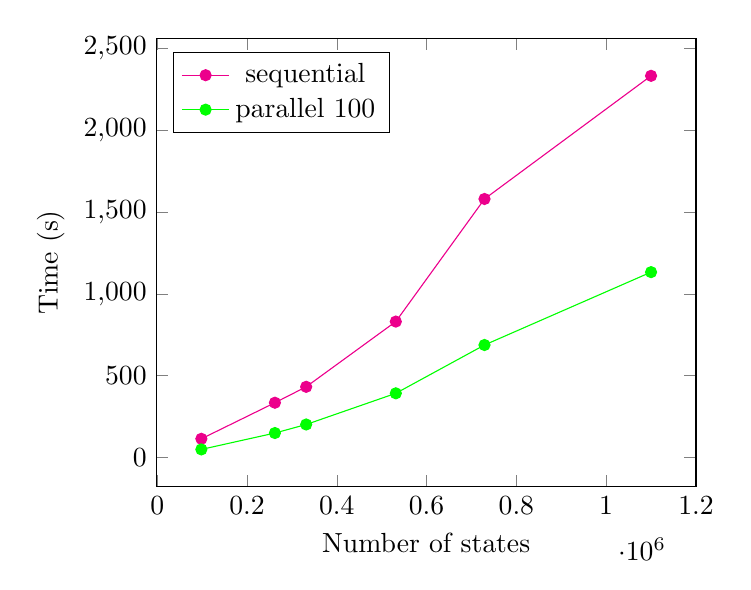
\begin{tikzpicture}
\definecolor{color0}{rgb}{0.75,0,0.75}

\begin{axis}[legend style={legend pos=north west},
ylabel={Time (s)},
xlabel={Number of states},
legend entries={{sequential},{parallel 100}}
% scaled ticks=false
]

% Sequential
\addplot [magenta, mark=*, mark size=2pt]
coordinates {
(98304,    113.690935000)
(262144,   334.272121000)
(331776,   431.582282000)
(531441,   830.441474000)
(729000,  1580.024665000)
(1099999, 2332.978991000)
};

% 100
\addplot [green, mark=*, mark size=2pt]
coordinates {
(98304,     48.798438000)
(262144,   148.977296000)
(331776,   201.183179000)
(531441,   391.800028000)
(729000,   687.234732000)
(1099999, 1132.697077000) % This is slightly over half an hr at 31 mins!
};

\end{axis}
\end{tikzpicture}
\caption{A comparison between the run-times of PIPE 5's sequential state space exploration algorithm and the new MapReduce-style parallel algorithm running on 4 cores for large Petri nets. This shows that the parallel implementation is consistently around twice as fast.}
\label{fig:pipe5_large_state_space}
\end{figure}